\section{Simulation, results and verification}

\subsection{Simulation}
In order to calculate the inside temperature of the house the model considers five heat flow. 

\begin{itemize}
    \item Transmission
    \item Ventilation
    \item Solar Gains
    \item Internal Heat Gains
    \item Heating/Cooling
\end{itemize}

The model also considers the mass of the air inside the house and the mass of the walls.  
House characteristics data.

The document Voorbeeldwoningen 2011 Bestaande bouw published by Agentschap NL \cite{VOORBEELD} will be used as a reference to determine the house characteristics. The document makes a classification of the house stock per construction type (7) and year of construction (4 time periods).  

\textbf{Construction type.}
\begin{itemize}
    \item Detached house (vrijstaande woning)
    \item Semi-detached house (2 onder 1 kap woning)
    \item Terraced house (rijwoning)
    \item Apartment block own access (maisonnettewoning)
    \item Apartment horizontal shared access (galerijwoning)
    \item Apartment block vertical shared access (portiekwoning)
    \item Apartment block in general (flatwoningen (overig))
    
\end{itemize}
\textbf{Year of construction.}
\begin{itemize}
    \item Build before 1964
    \item Build between 1965 and 1974
    \item Build between 1975 and 1991
    \item 	Build between 1992 and 2005
\end{itemize}

For the first model, the data of a detached house building build between 1975 and 1991 has been used. 
The energy consumption sum presented in the report as the first validation mechanism for this model. In the following model development, we should look for the possibility to validate the model with the use of real data.

\textbf{Climate data.}\\
NEN 5060:2008 and 2018 nl (Hygrothermische eigenschappen van gebouwen -Referentieklimaatgegevens), will be used as the climate data for the simulations.

\textbf{Internal heat gains data.}\\
There is no reference document about the internal heat gains for dwelling in the Netherlands. We can consider that there are two people living in the house with an average working schedule.
Control mechanism
The heating will be controlled by a thermostat. The indoor temperature of the house is based on recommendation given on the ISSO publication Kleintje Binnenklimaat. The indoor temperature should be maintained at a minimum of 20 degrees. 
We could consider taking cooling into account. 


\subsection{Results}
To test the model, we have used the data from the document Voorbeeldwoningen 2011 Bestaande bouw published by Agentschap NL \cite{VOORBEELD}. We have run the model for a detached house building build between 1975 and 1991 and for row house building build between 1975 and 1991.For the detached house the model calculates a sum of the yearly energy needs of 10545 kWh. The document Voorbeeldwoningen 2011 gives a calculated energy use for heating and hot water of 1542 m3 gas. The average gas consumption of hot tap water on a Dutch household is 300 m3gas. We assume a combustion (under) value ho=35.2 MJ/m3 gas. Taking into consideration a heating system efficiency of 0.9, the energy need is 10843 kWh. 


\begin{equation}
\frac{(1542-300) \cdot 35200}{3600\cdot 0.9}= 10843[KWh] 
\end{equation}


For the row house the model calculates a sum of the yearly energy needs of 19776 kWh. The sidewalls have been considered as adiabatic walls. The document Voorbeeldwoningen 2011 gives a calculated energy use for heating and hot water of 2616 m3 gas. The average gas consumption of hot tap water on a Dutch household is 300 m3gas. Taking into consideration a heating system efficiency of 0.9, the energy need is 20219 kWh. 

\begin{equation}
\frac{(2616-300) \cdot 35200}{3600\cdot 0.9}= 20129[KWh] 
\end{equation}

The results give an indication that the model is on the right result range for detached and row house.

The plot on figure \ref{fig:Simulationresults}, show the comparison of simulation results and annual heating consumption in Voorbeeldwoningen 2011 \cite{VOORBEELD}. More results can be found in Appendix B

\begin{figure}[H]
	\centering
	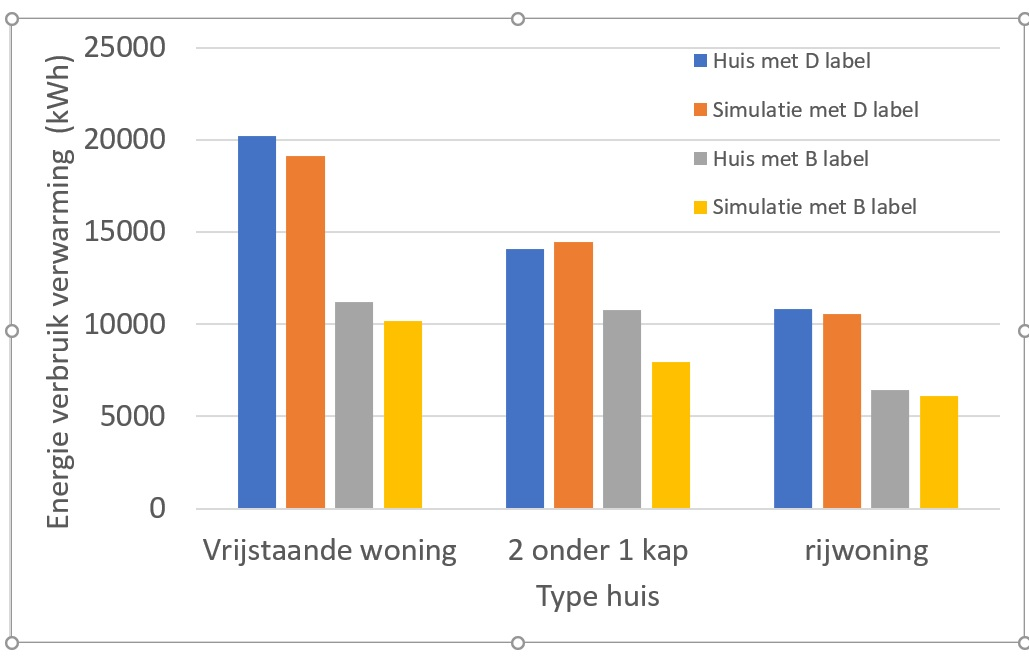
\includegraphics[width=1.0\columnwidth]{Pictures/Simulation results.jpg}
	\caption[Short title]{Simulation versus energy usage}
	\label{fig:Simulationresults}
	\end{figure}
\newpage

The graph in figure \ref{fig:heatingvstemp} shows the yearly heating demand needed for difference outdoor temperature.
It is clearly show the typical whether condition in the Netherlands where most of the energy use for heating happen at temperature range from 4 to 8 degree $^oC$.

\begin{figure}[H]
	\centering
	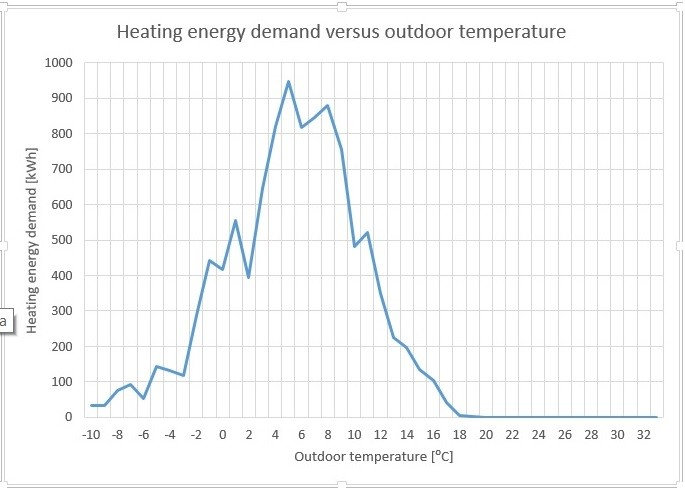
\includegraphics[width=1.0\columnwidth]{Pictures/Yearheatingdemand.jpg}
	\caption[Short title]{Simulation versus energy usage}
	\label{fig:heatingvstemp}
	\end{figure}
	
In order to get an estimation of the minimum heating power capacity needed to maintain a specific indoor temperature for the whole year the model thermostat has been set at a constant temperature day and night.
Minimum heating power capacity needed to maintain a specific indoor temperature has been shown in table 1.

\begin{table}[H]
    \centering
    \begin{tabular}{|c|c|}
    \hline
    Indoor temperature $[^oC]$  & Minimum heating powercapacity $[W]$ \\
    
    \hline
     18     &  6041 \\
     
     \hline
     19     &  6335 \\
     
     \hline
     20     &  6474 \\
     
     \hline
     21     &  6704 \\
     
     \hline
     22     &  6972 \\
     
     \hline
     23     &  7144 \\
     
     \hline
     24     &  7366 \\
     
    \hline

    \end{tabular}
    \caption{Minimum heating powercapacity}
    \label{tab:Minimumheat}
\end{table}
 
\newpage